\documentclass[a4paper,12pt]{article}
\usepackage[english,vietnamese]{babel}
\usepackage{amsmath}
\usepackage{amssymb}
\usepackage{booktabs}
\usepackage{lmodern}
\usepackage{graphicx}
\usepackage{hyperref}
\usepackage{lmodern}
\usepackage{forest}
\usepackage{textcomp}
\usepackage[nottoc,numbib]{tocbibind}

\renewcommand{\thefootnote}{\fnsymbol{footnote}}

\begin{document}
\setcounter{page}{0}
\thispagestyle{empty}
\vspace*{\stretch{1}}
\begin{flushright}
  \setlength{\baselineskip}{1.4\baselineskip}
\textbf{\Huge Midterm Report\\Sorting and Searching}
  \noindent\rule{\textwidth}{5pt}
  \emph{\Large Object Oriented Programming}
  \vspace{\stretch{1}}

  \textbf{by Nguyễn Công Thành, Nguyễn Gia Phong\\
          Nguyễn Văn Tùng, Trần Minh Vương and Trần Hồng Minh\\}
  \selectlanguage{english}
  \today
\end{flushright}
\vspace*{\stretch{2}}
\pagebreak

\selectlanguage{english}
\tableofcontents
\pagebreak

\section{Introduction}
\subsection{Brief Description}
Since the dawn of computer science, sorting and searching algorithms
have drawn a significant amount of attention from researchers,
due to their broad applications in solving a huge number of problems
and sub-problems in many fields.  In spite of their straightforward, familiar
statements, these algorithm link with a variety of important programming
concepts, namely data structures, divide and conquer technique and of course
complexity analysis and time–space tradeoffs.

In this report, we only discuss some of the most basic searching
and sorting algorithms.  While trying to implement them, we also analyze
their strengths and weaknesses, as well as the ease and difficulties
we encounter using the language Java and object-oriented programming in general.

Whilst overall, we follow~\cite{wu}, we also try to make use of newer Java
features to write more generic and concise code.

This report is licensed under a
\href{http://creativecommons.org/licenses/by-sa/4.0/}{Creative Commons
Attribution-ShareAlike 4.0 International License.}

\selectlanguage{vietnamese}
\subsection{Authors and Credits}

The work has been undertaken by group number 11, whose members are listed
in the following table, with Nguyễn Công Thành being our leader.
\begin{center}
  \begin{tabular}{c c}
    \toprule
    Full name & Student ID\\
    \midrule
    Nguyễn Công Thành & BI9-210\\
    Nguyễn Gia Phong & BI9-184\\
    Nguyễn Văn Tùng & BI9-229\\
    Trần Minh Vương & BI9-239\\
    Trần Hồng Minh & BI8-114\\
    \bottomrule
  \end{tabular}
\end{center}

We would like to express our special thanks to Dr. Nghiêm Thị Phương,
whose lectures gave us basic understanding on the key principles of
object-oriented programming.  Without her guidance, we might never
have a chance to take an in-depth exploration on this topic.
\pagebreak

\selectlanguage{english}
\section{Searching}
For the sake of simplicity, we only consider searching operating on array-like
data structures with constant-time random access and without duplicated entries.
This affects a few implementation design decision we will be making later on.
The searching problem is then stated in ~\cite[p.~634]{wu} accordingly:
\begin{quote}
  Given a value $x$, return the [zero-based] index of $x$ in the array,
  if such $x$ exists.  Otherwise, return \verb|NOT_FOUND| (-1).
\end{quote}

In this section, we will discover two searching algorithms: linear search
and binary search.  Both of these, albeit being simple, are being used in
many different programming tasks.

\subsection{Linear Search}
Linear search, by definition, sequentially checks each element of a list
until a match is found or the whole list has been searched.  This matches
the algorithm implemented in \verb|java.util.List.indexOf|~\cite[indexOf]{list}.
Given
\begin{verbatim}
var list = java.util.Arrays.asList(4, 20, 6, 9);
\end{verbatim}
where \verb|var| is a Java SE 10 feature for eliding ``the often-unnecessary
manifest declaration of local variable types''~\cite{var}, which, in this case,
is \verb|List<Integer>|.

\verb|list.indexOf(6)| would then give 2 and \verb|list.indexOf(7)| returns -1.

For the matter of completeness, we also try to implement the description
provided by the documentation~\cite[indexOf]{list}
\begin{verbatim}
import java.util.List;

public class Search
{
  public static final int NOT_FOUND = -1;

  public static linear(List l, Object o)
  {
    for (int i = 0; i < l.size(); ++i)
      if (o == null ? l.get(i) == null : o.equals(l.get(i)))
        return i;
    return NOT_FOUND;
  }
}
\end{verbatim}

From this dummy implementation, it is trivial that linear search has,
as it name suggests, \emph{linear time} complexity.  The nullity check
every iteration adds a bit of overhead, but if performance is ever concerned,
the better tested and optimized standard library should be used instead.
Moving \verb|o == null| to the upper level would require duplicating
the \verb|for| loop, creating redundancy and making the code less readable
and less maintainable.

Unsurprisingly, 2 and -1 are returned from
\verb|Search.linear(list, 6)| and \verb|Search.linear(list, 7)|,
respectively.

\subsection{Binary Search}
Binary search find the position of a target value within a sorted array by
``testing the middle of an interval, eliminating the half of the [array] in
which the key cannot lie, and then repeating the procedure iteratively''
\cite{bsearch}.  This could be intuitively implemented using recursion:
\begin{verbatim}
// ...
public class Search
{
  // ...
  private static <T>
  int binary(List<? extends Comparable<? super T>> list, T key,
             int low, int high)
  {
    if (high < low)
      return NOT_FOUND;
    var mid = (low + high) / 2;
    var cmp = list.get(mid).compareTo(key);
    if (cmp < 0)
      return binary(list, key, mid + 1, high);
    if (cmp > 0)
      return binary(list, key, low, mid - 1);
    return mid;
  }
}
\end{verbatim}

\verb|Search.binary| is declared as a \emph{generic method} to allow
more implicit calls, where the compiler will \emph{infer} the type of \verb|key|
as well as that of each element of \verb|list|~\cite{infer}.  This makes
the method work on any type of argument that is a subclass of \verb|Comparable|,
which is required for \verb|Comparable.compareTo|.  In fact,
\verb|java.util.Collections.binarySearch|'s declaration follows
the same strategy~\cite[binarySearch]{collections}.

Instead of directly exposing this method where users need to provide
the lower and higher bound of the indices, we overload it with a wrapper
to ensure encapsulation:
\begin{verbatim}
// ...
public class Search
{
  // ...
  public static <T>
  int binary(List<? extends Comparable<? super T>> list, T key)
  {
    return binary(list, key, 0, list.size());
  }
}
\end{verbatim}

To test our implementation, we first need \verb|list| to be sorted.
By providing \verb|null| to its \verb|sort| method, we can sort it
in the elements' natural (ascending) order~\cite[sort]{list}.
As \verb|list| is now [4, 6, 9, 20], \verb|Search.binary(list, 6)|
and \verb|Search.binary(list, 7)| return 1 and -1 respectively.

\verb|java.util.Collections.binarySearch(list, 7)| gives -3, however,
due to its slightly different behavior:
\begin{quote}
  [If \verb|key| is not in the list, returns] \verb|(-(insertion point) - 1)|.
  The insertion point is defined as the point at which the key would be
  inserted into the list: the index of the first element greater than the key,
  or \verb|list.size()| if all elements in the list are less than
  the specified key.~\cite[binarySearch]{collections}
\end{quote}

Since the algorithm only give up the search until the array is bisected to
a nonpositive length (\verb|high < low|), the time-complexity of binary search
is asymptotic to $\log_2 n$, where $n$ is the size of the array.
In other words, on modern 64-bit computers with support for at most 18EB
of address space, the running time is still negligible (64 comparisons).
Despite the use of \verb|List| interface in the implementation,
\verb|Search.binary| is not $\Theta(\lg n)$\footnote{The notation
$f = \Theta(g)$ indicates that $f$ grows at the same rate as $g$.}
on \verb|LinkedList|, which has $\Theta(n)$ random access.

Since the algorithm only works on ordered lists, it is not
suitable for iteratively inserting to a sorted list, as for linear
data structures, either random access or middle insertion has to be
$\Omega(n)$\footnote{The notation $f = \Omega(g)$ indicates that $f$ grows at
least as as fast as $g$.}.  In that case, self-balancing binary search tree
should be used instead.
\pagebreak

\section{Sorting}
The sorting problem is stated in~\cite[p. 638]{wu} as
\begin{quote}
  Given an array of $n$ values, arrange the values into ascending order.
\end{quote}

This section discusses only three sorting algorithms,
namely selection sort, bubble sort and heapsort.

\subsection{Selection Sort}
Selection sort could be performed by iterating through every position and select
the minimum element from the current one to the end of the array.  The in-place
algorithm could be implemented in Java as follows:
\begin{verbatim}
import java.util.List;

import static java.util.Collections.swap;

public class Sort
{
  public static <T extends Comparable<? super T>>
  void selection(List<T> list)
  {
    int i, j, m, n = list.size();
    for (i = 0; i < n; ++i)
      {
        for (m = j = i; j < n; ++j)
          if (list.get(j).compareTo(list.get(m)) < 0)
            m = j;
        swap(list, i, m);
      }
  }
}
\end{verbatim}

Since only atomic \verb|int|'s are introduced, the space complexity is
$\Theta(1)$.  The time complexity is, in term of swaps, $\Theta(n)$
and, in term of comparisons,
\[T(n) = \sum_{i=0}^{n-1}\sum_{j=i}^{n-1}1
       = \sum_{i=0}^{n-1}(n - i)
       = \sum_{i=1}^{n}i
       = \frac{n^2 + n}{2}
       = \Theta(n^2)\]

One could micro-optimize by tweaking \verb|i|'s and \verb|j|'s
bounds by an unit but that does not make the algorithm
any faster asymptotically.

Just to make sure everything works correctly, we do a simple check
\begin{verbatim}
var list = java.util.Arrays.asList("foo", "bar", "baz");
Sort.selection(list);
System.out.println(list);
\end{verbatim}
and get \verb|[bar, baz, foo]| printed to \verb|stdout| as expected.

\subsection{Bubble Sort}
In~\cite[p. 646]{wu}, the author praised bubble sort to finish sooner than
selection sort on average and best cases.  Whilst the latter is true,
we will try to explain why the former is generally incorrect.

To do this, we first need to understand what bubble sort is.
As defined in~\cite[p. 40]{clrs}, the code below operating on
an array \verb|a| of size \verb|n| qualifies as bubble sort.
\begin{verbatim}
for (int i = n - 1; i > 0; --i)
  for (int j = 1; j < i; ++j)
    if (a[j] < a[j - 1])
      swap(a, j, j - 1);
\end{verbatim}

This naïve version, like selection sort, has the time complexity $\Theta(n^2)$
in term of comparisons (it underperform selection sort in term of swaps
however--this will be discussed right after the implementation is completed).
Though, as pointed out in~\cite{bubblebad},
\begin{quote}
  Nearly every description of bubble sort describes
  how to terminate the sort early if the vector becomes sorted.
\end{quote}

Hence, we \emph{upgrade} the pseudocode to
\begin{verbatim}
boolean swapped;
do
  {
    swapped = false;
    for (int j = 1; j < n; ++j)
      if (a[j] < a[j - 1])
        {
          swap(a, j, j - 1);
          swapped = true;
        }
  }
while (swapped);
\end{verbatim}

We can do further optimization avoiding comparing the last $t - 1$ items
when running for the $t$-th time of the outer loop, as after iteration $t - 1$,
these have already \emph{bubbled up} to its final place~\cite{wikibubble}.
With this in mind, we write our final implementation:
\begin{verbatim}
// ...
public class Sort
{
  // ...
  public static <T extends Comparable<? super T>>
  void bubble(List<T> list)
  {
    for (int n = list.size(), m = 0; n > 1; n = m, m = 0)
      for (int i = 1; i < n; ++i)
        if (list.get(i).compareTo(list.get(i - 1)) < 0)
          swap(list, m = i, i - 1);
  }
}
\end{verbatim}

In the best case where the list is already sorted, during the first iteration
of the outer loop, \verb|m| remains zero, which is then assigned to \verb|n|
to break the loop, hence the time complexity is that of the inner loop
or $n - 1 = \Omega(n)$.  Otherwise, denote $S$ as a subset of all
positive integers not greater than \verb|list.size()|.  The time complexity
would then be
\[T(n) = \sum_{n\in S}\Theta(n)\]
On random data, $\#S = \Theta(n)$ and thus $T(n) = \Theta(n^2)$.

As demonstrated in~\cite{bubblebad}, selection sort outperforms bubble sort
on average cage, despite their asymptotically equivalent time complexity:
\begin{center}
  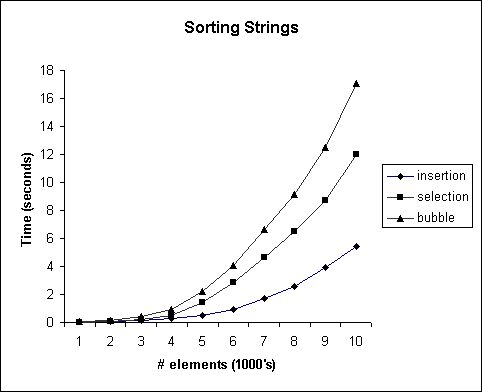
\includegraphics[width=0.57\textwidth]{bubbleplot.jpg}
\end{center}

Looking back at~\cite[p. 646]{wu}, we are now able to spot Wu's misconception:
\begin{quote}
  On average, we expect the bubble sort to finish sorting sooner than
  the selection sort, \emph{because there will be more data movements for
  the same number of comparisons}, and there is a test to exit the method
  when the array gets sorted.
\end{quote}

While bubble sort may take advantage of the pre-sorted parts of the array
to do fewer comparisons, the number of swaps is $\Theta(n^2)$, which grows
strictly faster than selection sort's $\Theta(n)$.  Consequently, instead of
swapping more to finish faster, the bubble variant does more unnecessary
data movements.  Furthermore, write operations on memory are usually slower
than reading, which makes swaps much costlier than comparisons.  Finally,
it could be summarized by a quote from Donald Knuth~\cite{peculiar},
\begin{quote}
  In fact, one of Demuth's main results was that in a certain sense
  `bubble sorting' is the optimum way to sort.  [...]  It turns out that
  [all other sorting methods studied] are always better in practice,
  in spite of the fact that Demuth has proved the optimality of bubble sorting
  on a certain peculiar type of machine. 
\end{quote}

\subsection{Heapsort}
Heapsort could be viewed as an improved version of selection sort, where
the selection is done on the right data structure: the heap~\cite{heapselect}.
To sort an array ascendingly in place, we use a binary max-heap to keep track
of the largest element in the unsorted region and move it to the beginning
of the sorted one, iteratively.

The binary heap is an array object $A$ which resembles a nearly completely
filled binary tree, except possibly the lowest level.  This kind of heap has
two attributes: $length$ of the array and $size$ of the heap,
where $0 \le size \le length$ and valid elements of the heap only reside
within the $[0, size)$ index interval of the array~\cite[p. 151]{clrs}.

We choose \verb|java.util.List| as the interface for the inner representation
of heap and come up with the following declaration:
\begin{verbatim}
import java.util.List;

public class Heap<T extends Comparable<? super T>>
{
  private List<T> list;
  private int size;
  public int getSize()
  {
    return size;
  }

  public int getLength()
  {
    return list.size();
  }

  public T get(int i)
  {
    return list.get(i);
  }
}
\end{verbatim}

Since the elements are of the type \verb|Comparable|, \verb|Heap| is a max-heap
in a purely conceptual sense.  That is, the order totally depends on
\verb|T.compareTo|, which could be defined or overridden by the users.
The max-heap property is then defined as that for every node $i$ other than
the root $A_0$, $A_{\mathrm{parent}(i)} \ge A_i$, where the indices of a node's
parent, left child and right child are given by
\[\begin{array}{ll}
  \mathrm{parent}(i) &= \left\lfloor\dfrac{i - 1}{2}\right\rfloor\\
  \mathrm{left}(i) &= 2i + 1\\
  \mathrm{right}(i) &= 2i + 2
\end{array}\]

To maintain this property at node $i$, with the assumption that
the binary trees rooted at left($i$) and right($i$) are already max-heaps,
we use \verb|heapify|, which sift the value at $A_i$ down the heap if it is
smaller than its children:
\begin{verbatim}
// ...
import static java.util.Collections.swap;

public class Heap<T extends Comparable<? super T>>
{
  // ...
  public void heapify(int i)
  {
    int right = i + 1 << 1;
    int left = right - 1;
    int largest = i;
    if (left < size && get(left).compareTo(get(largest)) > 0)
      largest = left;
    if (right < size && get(right).compareTo(get(largest)) > 0)
      largest = right;
    if (largest != i)
      {
        swap(list, i, largest);
        heapify(largest);
      }
  }
}
\end{verbatim}

At each call, the index of the greatest element among $A_i$,
$A_{\mathrm{left}(i)}$ and $A_{\mathrm{right}(i)}$ is assigned
to \verb|largest|.  In case $A_i$ is greatest, the subtree rooted at $A_i$
is already a max-heap and the method terminates.  Otherwise, $A_i$ is swapped
with $A_{\mathtt{largest}}$, which makes node $i$ and its children to satisfy
the max-heap property.  The subtree rooted at \verb|largest|, though,
\emph{might} violate the property so \verb|heapify| needs to be called on it.
For instance, given $i$ points to the subtree on the left, then \verb|heapify|
would step-by-step turn it to the one on the right:
\begin{center}
  \begin{forest}
    for tree={circle,draw}
    [,phantom [4,fill=yellow [9 [0] [6]] [8 [3] [,phantom]]]
              [9 [4,fill=yellow [0] [6]] [8 [3] [,phantom]]]
              [9 [6 [0] [4,fill=yellow]] [8 [3] [,phantom]]]]
  \end{forest}
\end{center}

The running time of \verb|heapify| on a subtree of height (number of edges
between the root and the furthest leaf) $h$ is the time $\Theta(1)$) to make
$A_i$, $A_{\mathrm{left}(i)}$ and $A_{\mathrm{right}(i)}$ a max-heap, plus
the time to run \verb|heapify| on one of its children if necessary:
\[T(h) \le T(h - 1) + \Theta(1)
       \le T(0) + \sum_{i=1}^{h}\Theta(1) = T(0) + \Theta(h)\]
Since $T(0)$ is obviously $\Theta(1)$,
\[T(h) \leq \Theta(h) \Longrightarrow T(h) = O(h)\footnotemark\]
A binary tree of size $n$ may have at maximum height of
$h = \lfloor\log_2 n\rfloor$, thus the time complexity with respect to
the size of the subtree is $O(\log_2 n)$.
\footnotetext{The notation $f = O(g)$ indicates that $f$ grows
at most as as fast as $g$.}

Noticeably, $\forall i \ge \lfloor n/2\rfloor,\; 2i + 2 > 2i + 1 \ge n
\iff \mathrm{right}(i) > \mathrm{left}(i) \ge n$.  In other words,
only nodes of indices less than $\lfloor n/2\rfloor$ have children.
Therefore, a heap could be constructed as follows
\begin{verbatim}
// ...
public class Heap<T extends Comparable<? super T>>
{
  // ...
  public Heap(List<T> a)
  {
    list = a;
    size = a.size();
    for (int i = size >> 1; i-- > 0;)
      heapify(i);
  }
}
\end{verbatim}

Before the construction, each node from $\lfloor n/2\rfloor$ (\verb|size >> 2|)
to $n - 1$ is a leaf and a trivial heap on its own.  Consider the iteration
where \verb|heapify| is called on node $i$ and assume every node after $i$
is the root of a heap beforehand, then after the iteration, all nodes from $i$
to $n - 1$ are foots of max-heaps.  Consequently, by mathematical induction,
after the construction, the whole array becomes a heap.  According
to~\cite[p. 159]{clrs}, this constructor runs in linear time ($O(n)$).

Heapsort uses the max-heap to select the next largest element to move it
to the start of the sorted region.  This in-place movement could be implemented
as the method \verb|pop|, which also return the largest element to make
the method make sense on its own.
\begin{verbatim}
// ...
public class Heap<T extends Comparable<? super T>>
{
  // ...
  public T pop() throws RuntimeException
  {
    if (size < 1)
      throw new RuntimeException("heap underflow");
    swap(list, 0, --size);
    heapify(0);
    return get(size);
  }
}
\end{verbatim}

Choosing the $n - 1$ largest element, we are left with the minimum value at
the beginning of the list and the rest of the list are all greater or equal to
the first element.
\begin{verbatim}
// ...
public class Sort
{
  // ...
  public static <T extends Comparable<? super T>>
  void heap(List<T> list)
  {
    var heap = new Heap<T>(list);
    for (int i = 1; i < list.size(); ++i)
      heap.pop();
  }
}
\end{verbatim}

The step-by-step selection from the example heap is shown below as
an illustration.  One may notice that the result qualifies as a min-heap.
\begin{center}
  \begin{forest}
    for tree={circle,draw}
    [,phantom [9 [6 [0] [4]] [8 [3] [,phantom]]]
              [8 [6 [0] [4]] [3 [9,edge=dotted] [,phantom]]]
              [6 [4 [0] [8,edge=dotted]] [3 [9,edge=dotted] [,phantom]]]]
  \end{forest}
\end{center}
\begin{center}
  \begin{forest}
    for tree={circle,draw}
    [,phantom [4 [0 [6,edge=dotted] [8,edge=dotted]]
                 [3 [9,edge=dotted] [,phantom]]]
              [3 [0 [6,edge=dotted] [8,edge=dotted]]
                 [4,edge=dotted [9,edge=dotted] [,phantom]]]
              [0 [3,edge=dotted [6,edge=dotted] [8,edge=dotted]]
                 [4,edge=dotted [9,edge=dotted] [,phantom]]]]
  \end{forest}
\end{center}

The running time of \verb|Sort.heap| is that of \verb|Heap| constructor,
plus $n - 1$ times that of \verb|Heap.pop|, which is
\begin{align*}
  T(n) &= O(n) + (n - 1)(\Theta(1) + O(\log_2 n))\\
       &= O(n) + \Theta(n)O(\log_2 n)\\
       &= O(n) + O(n\log_2 n)\\
       &= O(n\log_2 n)
\end{align*}
This is a huge improvement from selection sort's and bubble sort's $O(n^2)$.
\pagebreak

\section{Comparing}\label{sec:cmp}
Our implementations of searching and sorting algorithms in Java work on
any collection of data whose \emph{natural} order is specified, that is,
where elements implement \verb|Comparable|.  However, they does not cover
the case \emph{another} order is required, there is not any option to use
our current library other than subclassing every item with a different
\verb|compareTo| method, which, in every sense, is counter-intuitive.

In~\cite{wu}, Wu dedicated a whole ``Sample Development'' section to address
this issue and came up with the final solution of using the standard interface
\verb|java.util.Comparator|~\cite{cmp} which declare the method \verb|compare|.
We start with refactoring \verb|Sort.selection| to comply with this facility:
\begin{verbatim}
// ...
import java.util.Comparator;

public class Sort
{
  public static <T>
  void selection(List<T> list, Comparator<T> comparator)
  {
    int i, j, m, n = list.size();
    for (i = 0; i < n; ++i)
      {
        for (m = j = i; j < n; ++j)
          if (comparator.compare(list.get(j), list.get(m)) < 0)
            m = j;
        swap(list, i, m);
      }
  }
}
\end{verbatim}

To sort in reversed order, we can subclass \verb|Comparator|
anonymously~\cite{anon}
\begin{verbatim}
var list = java.util.Arrays.asList(4, 2, 0, 6, 9);
Sort.selection(list, new java.util.Comparator<Integer>()
{
  public int compare(Integer a, Integer b)
  {
    return -a.compareTo(b);
  }
});
System.out.println(list);
\end{verbatim}

As expected, the snippet above prints \verb|[9, 6, 4, 2, 0]| to \verb|stdout|.

In order to maintain backward-comparability, we write a helper class extracting
the natural order from any \verb|Comparable| to a \verb|Comparator|:
\begin{verbatim}
import java.util.Comparator;

public class Compare<T extends Comparable<? super T>>
implements Comparator<T>
{
  public int compare(T a, T b)
  {
    return a.compareTo(b);
  }
}
\end{verbatim}
and wrap the current \verb|Sort.selection| with
\begin{verbatim}
// ...
public class Sort
{
  // ...
  public static <T extends Comparable<? super T>>
  void selection(List<T> list)
  {
    selection(list, new Compare<T>());
  }
}
\end{verbatim}

\verb|Sort.bubble| can be refactored similarly, but since \verb|Sort.heap|
does all the comparisons in \verb|Heap|, we are required to make \verb|Heap|
work with \verb|Comparator|'s
\begin{verbatim}
// ...
import java.util.Comparator;

public class Heap<T>
{
  // ...
  private Comparator<T> cmp;

  public void heapify(int i)
  {
    int right = i + 1 << 1;
    int left = right - 1;
    int largest = i;
    if (left < size && cmp.compare(get(left), get(largest)) > 0)
      largest = left;
    if (right < size && cmp.compare(get(right), get(largest)) > 0)
      largest = right;
    if (largest != i)
      {
        swap(list, i, largest);
        heapify(largest);
      }
  }

  public Heap(List<T> a, Comparator<T> c)
  {
    list = a;
    size = a.size();
    cmp = c;
    for (int i = size >> 1; i-- > 0;)
      heapify(i);
  }
}
\end{verbatim}
and re-write \verb|Sort.heap| to use the new \verb|Heap|
\begin{verbatim}
// ...
public class Sort
{
  // ...
  public static <T>
  void heap(List<T> list, Comparator<T> comparator)
  {
    var heap = new Heap<T>(list, comparator);
    for (int i = 1; i < list.size(); ++i)
      heap.pop();
  }

  public static <T extends Comparable<? super T>>
  void heap(List<T> list)
  {
    heap(list, new Compare<T>());
  }
}
\end{verbatim}

For the next example, we use a minimal, read-only version of the \verb|Person|
class from~\cite[p. 666]{wu}, which is ordered by \verb|name| by default:
\begin{verbatim}
public class Person implements Comparable<Person>
{
  private String name;
  private Integer age;
  private Character gender;

  public Person(String name, Integer age, Character gender)
  {
    this.name = name;
    this.age = age;
    this.gender = gender;
  }

  public int compareTo(Person other)
  {
    return this.name.compareTo(other.name);
  }

  public String toString()
  {
    return String.format("%s (%d%c)", name, age, gender);
  }

  public String getName()
  {
    return name;
  }

  public Integer getAge()
  {
    return age;
  }
 
  public Character getGender()
  {
    return gender;
  }
}
\end{verbatim}

We use a list of the oldest current state leaders~\cite{old} for this test
\begin{verbatim}
var list = java.util.Arrays.asList(
  new Person("Mahathir Mohamad", 94, 'M'),
  new Person("Elizabeth II", 93, 'F'),
  new Person("Sheikh Sabah Al-Ahmad Al-Jaber Al-Sabah", 90, 'M'),
  new Person("Paul Biya", 86, 'M'),
  new Person("Michel Aoun", 84, 'M'),
  new Person("Mahmoud Abbas", 83, 'M'),
  new Person("Francis", 82, 'M'));
Sort.heap(list);
list.forEach(System.out::println);
\end{verbatim}
and get
\begin{verbatim}
Elizabeth II (93F)
Francis (82M)
Mahathir Mohamad (94M)
Mahmoud Abbas (83M)
Michel Aoun (84M)
Paul Biya (86M)
Sheikh Sabah Al-Ahmad Al-Jaber Al-Sabah (90M)
\end{verbatim}

It would neither be challenging to re-sort this list by their ages:
\begin{verbatim}
var ageComparator = new java.util.Comparator<Person>()
{
  public int compare(Person a, Person b)
  {
    return a.getAge().compareTo(b.getAge());
  }
};
Sort.heap(list, ageComparator);
list.forEach(System.out::println);
\end{verbatim}
which gives us
\begin{verbatim}
Francis (82M)
Mahmoud Abbas (83M)
Michel Aoun (84M)
Paul Biya (86M)
Sheikh Sabah Al-Ahmad Al-Jaber Al-Sabah (90M)
Elizabeth II (93F)
Mahathir Mohamad (94M)
\end{verbatim}

Linear search is able to run without any modification: we would still receive
4 from \verb|Search.linear(list, list.get(4))|.  Binary search, however,
would not work correctly if the order of the list is not \emph{natural}.
One with \verb|Comparator| support may be implemented as follows.
\begin{verbatim}
import java.util.List;
import java.util.Comparator;

public class Search
{
  // ...
  private static <T>
  int binary(List<? extends T> list, T key,
             Comparator<? super T> c, int low, int high)
  {
    if (high < low)
      return NOT_FOUND;
    var mid = (low + high) / 2;
    var cmp = c.compare(list.get(mid), key);
    if (cmp < 0)
      return binary(list, key, c, mid + 1, high);
    if (cmp > 0)
      return binary(list, key, c, low, mid - 1);
    return mid;
  }

  public static <T>
  int binary(List<? extends T> list, T key,
             Comparator<? super T> c)
  {
    return binary(list, key, c, 0, list.size());
  }
}
\end{verbatim}

Now \verb|Search.binary(list, list.get(5), ageComparator)| would return
the right index 5 instead of -1 like \verb|Search.binary(list, list.get(5))|.
\pagebreak

\section{Conclusion}
Albeit searching and sorting belong to the category of algorithms,
by implementing them, we were still able to recognize a variety of
object-oriented concepts, namely:
\begin{enumerate}
  \item Through encapsulation of the inner representations
    and behaviors, we can create intuitive programming interfaces,
    whilst keeping the code clear and concise.  Notable examples are
    the implementation of binary search and the heap data structure.
  \item Through polymorphism, generic and convenient libraries can be written,
    which allow more \emph{code reuse} and thus facilitate more effective
    development.  We wrote all of the classes and methods with this principle
    in mind.
  \item Through inheritance, it is possible to extend the functionalities of
    each object.  Together with polymorphism (which defines the behavioral
    interfaces), it enable us to generalize our codebase one step further,
    as shown in section~\ref{sec:cmp}, without spending too much energy
    on refactoring.
\end{enumerate}

Generally, though, we find shoving every self-contained function into a class
as a static method rather redundant.
\pagebreak

\begin{thebibliography}{99}
  \bibitem{wu} C. Thomas Wu.
    ``Chapter 11: Sorting and Searching''.
    \emph{An Introduction to Object-Oriented Programming with Java}, 5 ed.
    McGraw-Hill, 2010.  ISBN 978–0–07–352330–9.
  \bibitem{list} \href{https://docs.oracle.com/javase/8/docs/api/java/util/List.html}{List (Java Platform SE 8)}.
    \emph{Oracle}.
  \bibitem{var} \href{http://openjdk.java.net/jeps/286}{JEP 286: Local-Variable Type Inference}.
    \emph{OpenJDK}.
  \bibitem{bsearch} \href{http://mathworld.wolfram.com/BinarySearch.html}{Binary Search}.
    \emph{Wolfram WathWorld}.
  \bibitem{infer} \href{https://docs.oracle.com/javase/tutorial/java/generics/methods.html}{Generic Methods}.
    \emph{Oracle}.
  \bibitem{collections} \href{https://docs.oracle.com/javase/8/docs/api/java/util/Collections.html}{Collections (Java Platform SE 8)}.
    \emph{Oracle}.
  \bibitem{clrs} Thomas H. Cormen, Charles E. Leiserson,
                 Ronald L. Rivest and Clifford Stein.
    \emph{Introduction to Algorithms}, 3 ed.
    MIT Press, 2009.  ISBN 978-0-262-03384-8.
  \bibitem{bubblebad} Owen Astrachan.
    \emph{\href{https://users.cs.duke.edu/~ola/bubble/bubble.html}{Bubble Sort: An Archaeological Algorithmic Analysis}}.
    Duke University.
  \bibitem{wikibubble} \href{https://en.wikipedia.org/wiki/Bubble_sort#Optimizing_bubble_sort}{Bubble sort}.
    \emph{Wikipedia}.
    Section 2.2: \emph{Optimizing bubble sort}.
  \bibitem{peculiar} Donald E. Knuth.  The Dangers of Computer-Science Theory.
    \emph{Studies in Logic and the Foundations of Mathematics}, vol. 74.
    Elsevier, 1973.
    doi:\href{https://doi.org/10.1016/S0049-237X(09)70357-X}{10.1016/S0049-237X(09)70357-X}.
  \bibitem{heapselect} Steven Skiena.
    ``Searching and Sorting''.
    \emph{The Algorithm Design Manual}, p. 109.
    Springer, 2008.
    doi:\href{https://doi.org/10.1007/978-1-84800-070-4_4}{10.1007/978-1-84800-070-4{\_}4}.
    ISBN 978-1-84800-069-8.
  \bibitem{cmp} \href{https://docs.oracle.com/javase/8/docs/api/java/util/mparator.html}{Comparator (Java Platform SE 8)}.
    \emph{Oracle}.
  \bibitem{anon} \href{https://docs.oracle.com/javase/tutorial/java/javaOO/anonymousclasses.html}{Anonymous Classes}.
    \emph{Oracle}.
  \bibitem{old} \href{https://en.wikipedia.org/wiki/Lists_of_state_leaders_by_age#10_oldest_currently_serving_state_leaders}{Lists of state leaders by age}.
    \emph{Wikipedia}.
    Section 1: \emph{10 oldest currently serving state leaders}.
\end{thebibliography}
\end{document}
